\section{Fine-tuning}

As a warmup, we will perform perhaps the most straightforward form of $k$-shot learning with a pre-trained model: directly fine-tuning the entire model on the $k$ examples. We will use two different sizes of smaller BERT models that have been compressed through distillation.\footnote{See \href{https://arxiv.org/pdf/1908.08962.pdf}{here} to learn more about this class of distilled BERT models. For final projects involving language models, these smaller BERT models may be useful for performing compute-friendly experiments!}

\begin{enumerate}[label={1.\alph*}]
    \item \points{2a} {\bf Implement In-Context Learning}

Complete the code for in-context learning in \texttt{icl.py}.
\begin{enumerate}[label=(\roman*)]
    \item Implement prompt creation for the XSum and bAbI tasks, which is found in \texttt{icl.py:get\_icl\_prompts()}. You will implement 4 prompt format modes:
    \begin{enumerate}[label={\arabic*}]
        \item \texttt{qa} \textbf{[only for bAbI]}: Add ``\texttt{ In the }'' after the question (including the final test question that we want to generate an answer for!) and before each answer, since this task involves answering questions about the physical whereabouts of a person. In addition, add a period after the answer (omitting the period can significantly impact your results!). Be sure to include a space between the question and \texttt{In the}, as well as a space before the answer (though keep in mind Note 1!). Note the  \texttt{Q:} and \texttt{A:} prompts in the example earlier don't apply here.
        \item \texttt{none} \textbf{[only for XSum]}: In this case, we use the raw $k$ examples without any additional formatting; that is, we just concatenate $[x_1; y_1; ... ; \allowbreak x_k; y_k; x^*]$ with a space between each element (but no space at the end), where $x^*$ is the input that we want to generate an answer for.
        \item \texttt{tldr} \textbf{[only for XSum]}: Add the text ``\texttt{ TL;DR: }'' after each article/input (including the final test article) and before the summary/target.
        \item \texttt{custom} \textbf{[only for XSum]}: Come up with your own prompt format for article summarization (different from the ones we've shown!).
    \end{enumerate}
    In general, the idea of in-context learning is to format the support examples in the same way as the test example, to leverage the model's tendency toward imitation.

    \textbf{Note 1: Due to a quirk with GPT-2 tokenization, you should not include a space at the end of your prompt before generation.}
    
    \textbf{Note 2: Be sure to shuffle the order of the support inputs/targets when you construct the prompt (we will need this randomization later).}
    \item Implement greedy sampling in \texttt{icl.py:do\_sample()}. The GPT-2 models used in this and the following questions use an autoregressive factorization of the probability of a sequence, i.e. $p_\theta(\mathbf{x}) = \prod_t p_\theta(x_t \mid x_{<t})$. `Greedy' sampling means that given a context $x_{<t}$ producing a distribution over next tokens $p_\theta(x_t \mid x_{<t})$, we deterministically choose the next token $x_t$ to be the token with highest probability.
    
    \textbf{Note 3: Be sure you understand what each dimension of the model's output \texttt{logits} represents. Misinterpreting the dimensions of this output can lead to subtle bugs.}
    
    \item Finally, put the pieces together by completing the implementation of \texttt{icl.py:\allowbreak run\_icl()}, using your \texttt{get\_icl\_prompts()} and \texttt{do\_sample()} functions, as well as the HuggingFace tokenizer defined in the loop. \\ \emph{Hint}: Your solution here should be less than 5 lines of code.
\end{enumerate}
    \item {\bf Observe Fine-Tuning}

\begin{enumerate}[label=(\roman*)]
    \item \points{1bi} {\bf Run Fine-Tuning}

Run the command:
    
{\small\texttt{python3 main.py --task run\_ft --model bert-tiny,bert-med --dataset amazon --k 1,8,128}}

to fine-tune two sizes of BERT models on the Amazon Reviews dataset for various values of $k$. While debugging, you can pass only one value for each of the arguments to run only that subset, e.g. \texttt{python3 main.py --task run\_ft --model bert-tiny --dataset amazon --k 1}.

If you see a log message like \texttt{Some weights of the model checkpoint...}, this is expected, since the pre-trained model does not contain a prediction head for our task (this is why we need to fine-tune!).

To plot your results, run the command:

{\small\texttt{python3 main.py --task plot\_ft --model bert-tiny,bert-med --dataset amazon --k 1,8,128}}

Your plot should look as follows:
\begin{center}
    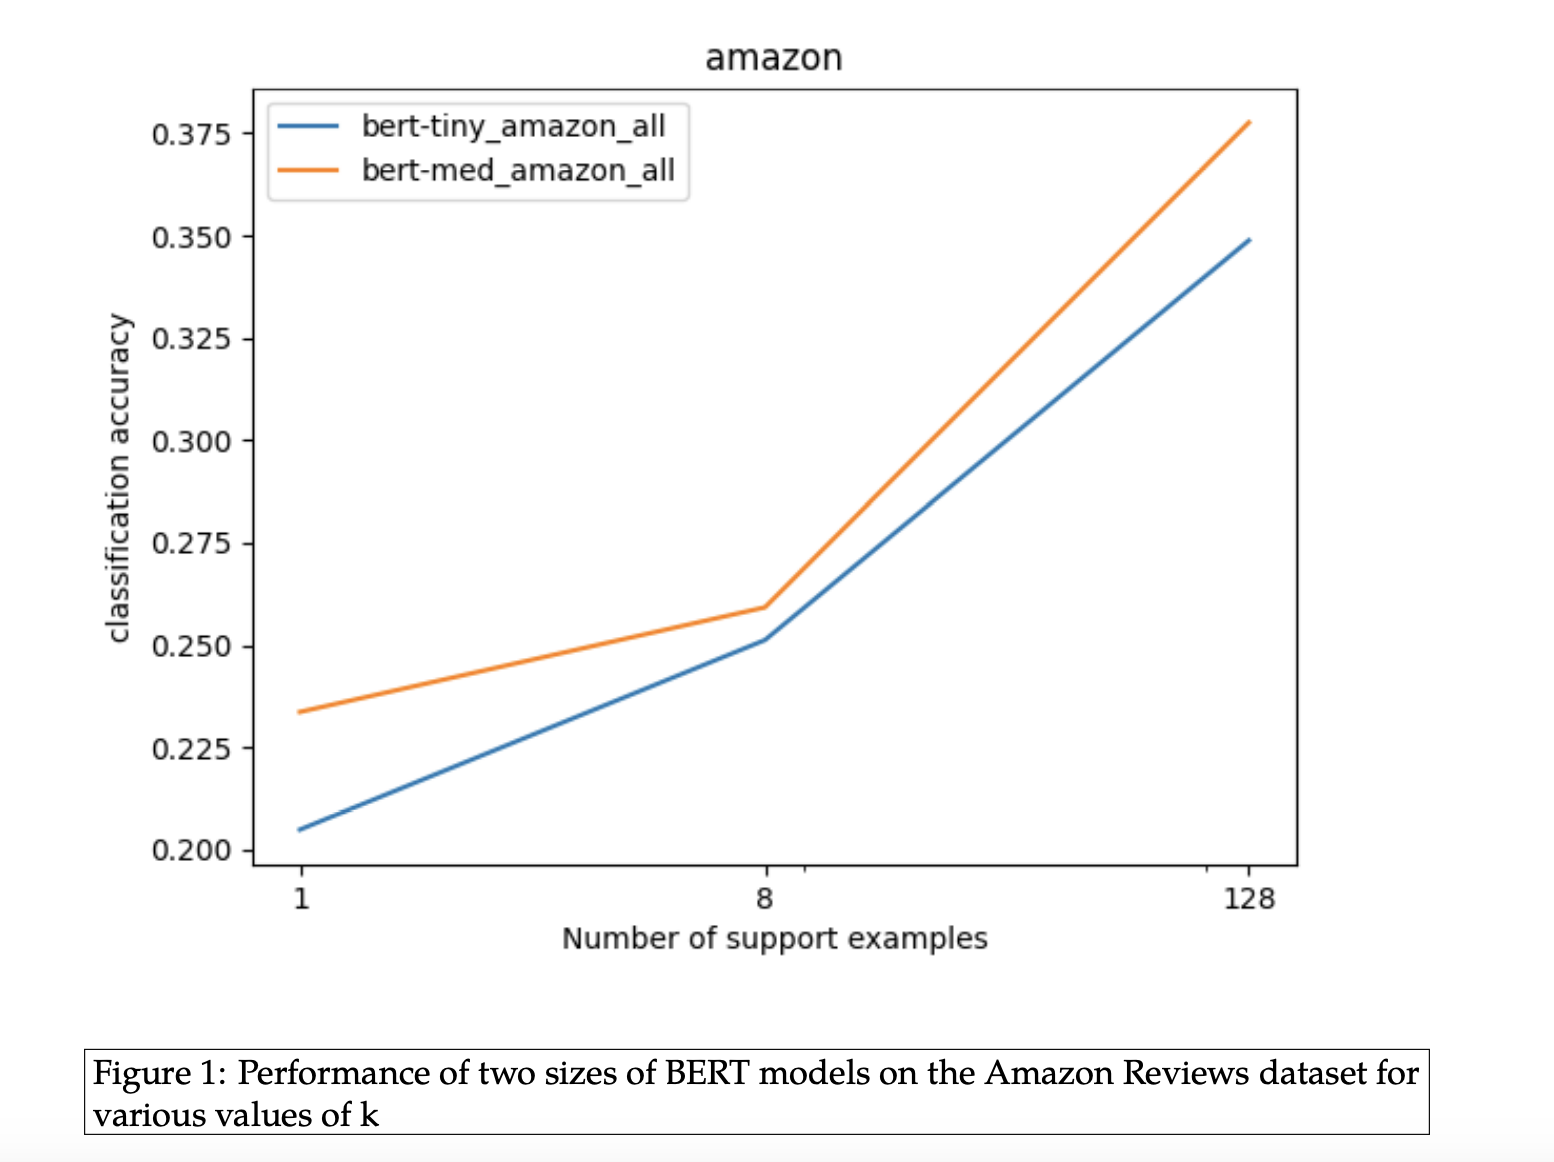
\includegraphics[width=0.75\linewidth]{./figures/finetune-1b}
\end{center}

\clearpage

    \item \points{1bii} {\bf Reason on Fine-Tuning}

In one sentence, what do you notice about the performance of the two model scales?

\clearpage

\end{enumerate}

\clearpage

    \item \points{1c} {\bf Storage for Fine-Tune}

If we fine-tune the all of our model parameters for each task, we must save a new complete copy of the model's parameters for each new task. As an example, a BERT-mini model similar to the ones you just fine-tuned has approximately 11.2 million parameters; assuming parameters are represented as 4-byte floats, after fine-tuning on a new task, how much disk space do we need to store the new fine-tuned model parameters?
    \item \points{1d} {\bf Disk Space}

Google's recent large language model \href{https://storage.googleapis.com/pathways-language-model/PaLM-paper.pdf}{PaLM} has 540 billion parameters. How much disk space would be needed to store a new fine-tuned version of this model, assuming parameters are represented as 4-byte floats?
\end{enumerate}